%!TEX program = xelatex
%\documentclass[pra,twocolumn]{revtex4-1}
%\documentclass[preprint]{revtex4-1}
% \documentclass[a4paper]{article}
% \usepackate{cite}
\documentclass[11pt,a4paper]{article}
\usepackage{fontspec,amsmath,amssymb,bm}
\usepackage{xeCJK}
\usepackage{graphics,graphicx,float,subfigure}
\usepackage{url}
\usepackage[margin=2cm]{geometry}
\usepackage{listings}
\usepackage{lmodern}            % Use latin modern fonts
\usepackage{authblk}
\usepackage{SIunits}
\usepackage{braket}
\usepackage{todonotes}
\setmonofont{DejaVu Sans Mono}
\setCJKmainfont{cwTeX Q Ming}
% for chinese document
\renewcommand{\figurename}{圖}
\renewcommand{\tablename}{表格}

\title{Title}
\author{彭陸}
\affil[1]{國立台灣大學物理系}
\date{\today}
%\affiliation{National Taiwan University}

\begin{document}
\maketitle
\begin{abstract}
%TODO: find CPT paper G. Alzetta, A. Gozzini, M. Moi, and G. Orriols, Nuovo Ci- mento Soc. Ital. Fis., B 36,5 1976.
We investigate the coherent population trapping (CPT) signal excited by train of ultrashort pulses in $D_1$ and $D_2$ optical absorption spectrum of Cesium atoms as well as simplified three, four and five-level systems with trap states. Using the Liouville formalism, we develop an algorithm which can calculate temporal evolution as well as steady state of the density matrix of an ensemble of cesium atoms. The line width and contrast of the comb CPT signal caused by pulse laser is compared to continuous wave (CW) CPT signal. It is shown that average laser power has smaller impact on the line width and light shift of comb CPT signal than on CW CPT signal. Therefore, we proposed that comb CPT signal can be used as a precise atomic frequency standard which is independent of laser power. Also, the line width of comb CPT signal is shown to be proportional to ground state relaxation rate $\gamma$.\\
\end{abstract}

\listoftodos
\section{Introduction}
The phenomenon that two ground states coupled to a common excited state by optical field is called coherent population trapping. It is observed first by Alzetta et al.\cite{Alzetta1976}. The phenomenon has been proposed for applications in the fields of atom cooling, magnetometry, lasing without inversion, and atomic frequency standards. We are especially interested in the application of CPT as atomic clock signal. CPT can be used as precise clock signal \cite{Vanier2005}\todo{Review some CPT clock research}. CPT phenomenon can be excited by both ultra fast pulse laser or two CW lasers. We are interested in the difference between comb CPT and CW CPT signals and the potential application of comb CPT signal.\\

In this paper, we first discuss the principle of CPT phenomenon and how the CPT phenomenon can be simplified using three-level, four-level or five-level systems with trap states, depending on the system's state diagram structure. Then we introduced the $D_1$ and $D_2$ optical absorption spectrum which are used in this paper.\\

In the second part of this paper, an perturbation algorithm we developed and used to calculate the temporal evolution and steady state of the density matrix of an ensemble of cesium atoms is presented. Using Liouville formalism, a super operator that operate on the density matrix can be calculated, which represent the temporal evolution of the density matrix caused by the optical pulse during the time segment between two adjacent pulses. The temporal evolution of density matrix can be calculated using this super operator.\\

In the last section, we make use of our algorithm to calculate comb CPT signal in both simplified model and system with all Zeeman sublevels taking into account. It is shown that simplified models present qualitative similar behavior as full Zemman sublevels calculation. We also compared the characters of comb CPT signal with CW CPT's. It is shown that laser power has much smaller influence on the line width and light shift of the CPT signal when using pulse laser. Therefore we propose that comb CPT signal can be used as an objective precise atomic frequency standard.\\

% who have calculated ? Focus on what? Why we calculate this? how repetition rate effect CPT, clock standard. different focus. objective frequency. light shift, bandwidth.

\section{Theory}
\subsection{Coherent Population Trapping (CPT)}
Coherent population trapping (CPT) is accomplished by applied two laser field in a $\Lambda$ scheme. The phenomenon can easily be observed in  alkali-metal atom. In the case of alkali atoms, the fields are applied to an ensemble of atoms in resonance with the transitions between the two hyperfine levels of the $S_{1/2}$ ground state and one of the $P$-state hyperfine levels, forming a $\Lambda$ scheme. When the frequency of the two laser is resonant with ground level and the P state, an interference occurs and the atoms can no longer absorb energy from the lasers. This is called the continuous wave CPT. The phenomenon, as observed at a hyperfine frequency, was first reported by Alzetta et al. in sodium by means of a multi-mode dye laser\cite{Alzetta1976}. Theoretical analysis of the phenomenon was developed by Orriols \cite{Orriols1979}. The system discussed in this article consist cesium atoms and two coherent radiation fields resonant with the transition from the levels $F=3$ and $F=4$ of the ground state to one of the hyperfine levels of the excited $P$ state. If level $P_{1/2}$, $F=3$ and $F=4$ is choose it is called $D_1$ radiation. If the $P$ state is $P_{3/2}$, $f=2$, $F=3$, $F=4$ and $F=5$, it is called $D_2$ radiation. Then scheme is showed in figure \missingfigure{Add a figure of d1 d2 line}.\\

In the present paper, right hand circular polarization exciting $\Delta m_F = +1$ is used. With no magnetic field is applied, all Zeeman levels must be considered. Even with magnetic field, all Zeeman levels may still play a role in the system evolution. Decay from the excited state takes place to all ground state Zeeman levels due to spontaneous emission and atomic collisions when a buffer gas is used. The atoms may be trapped in level $m_F = +4$ or $m_F = -4$ depending on the polarization used. In this case, these atoms no longer belong in the $\Lambda$ scheme, it is necessary to add trap states to the system in order to model the phenomenon\cite{Vanier1998}. For the $D_1$ system. figure \ref{fig:four_level} shows the $\Lambda$ scheme of cesium $D_1$ line system with circular polarized ($\sigma = +1$) CW laser. Atoms accumulate in their decay to the level $F=4,m_F=4$, as it is not connected by radiation to any $P_{1/2}$ state. The atoms then slowly redistribute to other Zeeman levels at the ground state relaxation rate $\gamma$. This state therefore is act like a ``leaky trap state''. A cesium $D_2$ level diagram is shown in figure \ref{fig:five_level}, beside the leaky trap state, there is another state $F=5.m_F=5$ which is linked to the trap state via radiation. Therefore one more state is added to the simplified model, forming a five level model.\\

The analysis is best done in the density-matrix formalism. The rate equations for the populations of the levels are obtained from Liouville—von Neumann equation:
\begin{equation}
  \label{eq:lvn}
  \frac{\partial \rho}{\partial t} = \frac{i}{i\hbar} \left[ H,\rho \right]
\end{equation}
\todo{Add Hamiltonian here}

\begin{figure}[H]
  \centering
  \subfigure[Three level system]{
    \includegraphics[width=0.2\textwidth]{small_system/three.pdf}
  \label{fig:three_level}
    }
  \subfigure[Four level system]{
    \includegraphics[width=0.2\textwidth]{small_system/four.pdf}
  \label{fig:four_level}
    }
  \subfigure[Five level system]{
    \includegraphics[width=0.2\textwidth]{small_system/five.pdf}
  \label{fig:five_level}
   }
   \caption{analogue of four and five level system}
   \label{fig:analog}
 \end{figure}

 The laser fields applied can be two continuous wave lasers or one pulse (frequency comb) laser. Because a frequency comb laser contain broad frequency range of frequency combs, the laser field can interact with every Zeeman sublevels even when magnetic field is applied. In the case or continuous wave laser, the CPT signal is called the CW CPT signal; in the case of pulse laser, the CPT signal is called the comb CPT signal. The CW CPT signal can be calculated easily using rotating wave approximation \cite{Vanier1998}\cite{Orriols1979}. The coherent accumulation processes in three-level model excited by pulse laser is calculated by Felinto et al. in 2004\cite{Felinto2004}. In this paper we extended the calculation to cesium atom's $D_1$ line (32 levels) and $D_2$ line (48 levels) and compare the results with CW CPT signal.\\

 \subsection{Cesium $D_1$ and $D_2$ optical absorption spectrum}
 To calculate the comb CPT signal more accurately, all Zeeman sublevels should be considered, since they all interact with the broad band frequency comb. There are two components of Cesium D-line; the $D_1$ line (the $6^2s_{1/2}}\Rightarrow6^2P_{1/2}$ transition) and $D_2$ line (the $6^2S_{1/2}\Rightarrow6^2P_{3/2}$ transition). The $D_2$ transition is more important to current atom optics research, because it has a cycling transition that is used for cooling and trapping cesium.\\

The decay rate $\Gamma$ which represent the natural line width (FWHM) of D-line components are $2\pi \cdot 4.575(12) \mega\hertz$ and $2\pi \cdot 5.234(13) \mega\hertz$ for $D_1$ transition and $D_2$ transition respectively. Because buffer gas is added in experiments, the decay rate $\Gamma$ is set to $700 \mega\hertz$ for both $D_1$ and $D_2$ transition in the simulation to fit the experimental condition.\todo{reference}\\

The off diagonal terms in the Hamiltonian represent the strength of the interaction between cesium and the nearly-resonant optical radiation, which is characterized by the dipole matrix elements. $\Braket{F m_F | er | F^{\prime} m_F^{\prime}}$ denotes the matrix element between two hyperfine sublevels $\ket{ F m_F }$ and $\ket{ F^{\prime} m_F^{\prime}}$. These dipole matrix element can be calculated using Wigner-Eckart theorem
\begin{equation}
  \Braket{ F m_F | er | F^{\prime} m_F^{\prime}} =\dots
\end{equation}

The following equation is the master equation for the density matrix of a $F_g \Rightarrow F_e$ hyperfine translation \cite{Steck2003}.
\begin{widetext}
\begin{align}
  \frac{\partial}{\partial t} \tilde{\rho}_{\alpha m_{\alpha},\beta m_{\beta}} = &
    - \frac{i}{2} \left[ \delta_{\alpha e}\sum_{m_g} \Omega \left( m_{\alpha},m_g \right) \tilde{\rho}_{g m_g, \beta m_{\beta}} - \delta_{g \beta}\sum_{m_e} \Omega \left( m_{e},m_\beta \right) \tilde{\rho}_{\alpha m_\alpha, e m_{e}} \right.\nonumber\\ &+ \left. \delta_{\alpha g}\sum_{m_e} \Omega^{\star} \left( m_{e},m_\alpha \right) \tilde{\rho}_{e m_e, \beta m_{\beta}} - \delta_{e \beta}\sum_{m_g} \Omega^{\star} \left( m_{\beta},m_g \right) \tilde{\rho}_{\alpha m_\alpha, g m_{g}} \right] \label{eq:masterpumpfield}   \\
 &-\delta_{\alpha e}\delta_{e \beta} \Gamma \tilde{\rho}_{\alpha m_{\alpha}, \beta m_{\beta}} \label{eq:masterdissipation1}\\
  &- \delta_{\alpha e}\delta_{g \beta} \frac{\Gamma}{2} \tilde{\rho}_{\alpha m_{\alpha},\beta m_{\beta}}\label{eq:masterdissipation2}\\
  &- \delta_{\alpha g}\delta_{e \beta} \frac{\Gamma}{2} \tilde{\rho}_{\alpha m_{\alpha}, \beta m_{\beta}} \label{eq:masterdissipation3}\\
  &+ \delta_{\alpha g}\delta_{g \beta} \Gamma \sum_{q = -1}^{1} \left[ \tilde{\rho}_{e \left( m_{\alpha} + q \right), e \left(m_{\beta}+q  \right)} \braket{F_e \left( m_{\alpha}+q \right) | F_g 1 m_{\alpha} q} \braket{  F_e \left( m_{\beta} + q \right)  | F_g 1 m_{\beta} q }\right]\label{eq:masterdissipation4}\\
  &+ i \left( \delta_{\alpha e} \delta_{g \beta} - \delta_{\alpha g}\delta_{e \beta} \right) \Delta\tilde{\rho}_{\alpha m_{\alpha}, \beta m_{\beta}} \label{eq:masterfreeevolution}\\
  &- \gamma (\delta_{\alpha,S_{1/2}F=3}\delta_{\beta,S_{1/2}F=4}+\delta_{\alpha,S_{1/2}F=4}\delta_{\beta,S_{1/2}F=3}) \tilde{\rho}_{\alpha m_{\alpha}, \beta m_{\beta}}\label{eq:groundstaterelax}\\
  &- \gamma \delta_{\alpha,S_{1/2}F=3}\delta_{\beta,S_{1/2}F=3} \sum_{m_{S_{1/2}F=4}} (\tilde{\rho}_{\alpha m_{\alpha}, \beta m_{\beta}} - \tilde{\rho}_{S_{1/2}F=4 m_{S_{1/2}F=4},S_{1/2}F=4 m_{S_{1/2}F=4} })\label{eq:groundstaterelax2}\\
  &- \gamma \delta_{\alpha,S_{1/2}F=4}\delta_{\beta,S_{1/2}F=4} \sum_{m_{S_{1/2}F=3}} (\tilde{\rho}_{\alpha m_{\alpha}, \beta m_{\beta}} - \tilde{\rho}_{S_{1/2}F=3 m_{S_{1/2}F=3},S_{1/2}F=3 m_{S_{1/2}F=3} })\label{eq:groundstaterelax3}
\end{align}
\end{widetext}


Equation \ref{eq:masterpumpfield} contain terms related to pump field, In this equation $\alpha$ and $\beta$ represent the hyperfine levels, $e$ means excited states ($P$ states), $g$ means ground states ($S$ states). The equations \ref{eq:masterdissipation1} to equation \ref{eq:masterdissipation4} are dissipation terms. Equation \ref{eq:masterfreeevolution} is the free evolution. Equations \ref{eq:groundstaterelax} to \ref{eq:groundstaterelax3} are terms related to ground state relaxation (PRINCIPLE OF GROUND STATE RELAX). $\Omega$ is the Rabi frequency between two magnetic sublevels. And $\tilde{\rho}_{\alpha\beta} \equiv \rho_{\alpha\beta} \exp \left( -i \Delta_{\alpha\beta} t \right)$ is a ``slowly varying coherence'', where $\Delta_{\alpha\beta}$ is the resonance frequency between state $\alpha$ and state $\beta$. $\rho$ is anti-symmetry, which means $\tilde{\rho}_{\alpha\beta} = \tilde{\rho}^{\ast}_{\alpha\beta}$. In general, the master equation is hard to treat analytically, a numerical solution of the time-dependent equation can be time-consuming if a large number of degenerate states are involved.\\

In the following discussions, we present a way to calculate both temporal evolution and steady state of the density matrix of an ensemble of cesium atoms interacting with femto-second pulse laser.

\subsection{Liouvillian formalism}
To calculate the time evolution of the density matrix, we use the Liouvillian formalism. Using the algorithm described below, a super operator (Liouville operator, tetradic matrix) that represent the time evolution of the density matrix during the time segment between adjacent laser pulses can be obtained. As an operator act on a state vector in a $n$-dimensional Hilbert space, a super operator is a mathematical transformation between operators in a $n^{2}$-dimensional Liouville space. For example, an $n \times n$ operator $\hat{A}$, in a $n$-dimensional Hilbert space $\mathcal{H}_{n}$

\begin{equation}
\hat{\mathcal{A}} =
 \begin{bmatrix}
  \braket{ 1 | \hat{A}|1 } & \braket{ 1 | \hat{A}|2 } & \cdots & \braket{ 1 | \hat{A}|n } \\
  \braket{ 2 | \hat{A}|1 } & \braket{ 2 | \hat{A}|2 } & \cdots & \braket{ 2 | \hat{A}|n } \\
  \vdots  & \vdots  & \ddots & \vdots  \\
  \braket{ n | \hat{A}|1 } & \braket{ n | \hat{A}|2 } & \cdots & \braket{ n | \hat{A}|n }
 \end{bmatrix}
\end{equation}

$\hat{\mathcal{A}}$ is represent as a vector with $n^2$ elements in a $n^2$-dimensional Liouville space $\mathcal{L}_{n^2}$
\begin{equation}
\hat{\mathcal{A}} =
 \begin{bmatrix}
  \braket{ 1 | \hat{A}|1 }\\
  \braket{ 1 | \hat{A}|2 }\\
  \braket{ 1 | \hat{A}|3 }\\
  \vdots\\
  \braket{ 1 | \hat{A}|n }\\
  \braket{ 2 | \hat{A}|1 }\\
  \vdots\\
  \braket{ n | \hat{A}|n }\\
 \end{bmatrix}
\end{equation}

With this vector representation of the operator in $\mathcal{L}_{n^2}$. The operator can be transformed using a $n^2 \times n^2$ matrix $\hat{\mathcal{S}}$ represented in $\mathcal{L}_{n^2}$, with $n^4$ independent elements. $\hat{\mathcal{S}}$ is called the super operator, Liouville operator or tetradic matrix.

\begin{equation}
\hat{\mathcal{S}} \left[ \hat{\mathcal{A}} \right] = \hat{\mathcal{B}}
\end{equation}

\begin{equation}
\footnotesize
 \begin{bmatrix}
  \braket{ 1 | \hat{S}|1 } & \braket{ 1 | \hat{S}|2 } & \cdots & \braket{ 1 | \hat{S}|n^2 } \\
  \braket{ 2 | \hat{S}|1 } & \braket{ 2 | \hat{S}|2 } & \cdots & \braket{ 2 | \hat{S}|n^2 } \\
  \vdots  & \vdots  & \ddots & \vdots  \\
  \braket{ n^2 | \hat{S}|1 } & \braket{ n^2 | \hat{S}|2 } & \cdots & \braket{ n^2 | \hat{S}|n^2 }
 \end{bmatrix}
 \begin{bmatrix}
  \braket{ 1 | \hat{A}|1 }\\
  \braket{ 1 | \hat{A}|2 }\\
  \braket{ 1 | \hat{A}|3 }\\
  \vdots\\
  \braket{ 1 | \hat{A}|n }\\
  \braket{ 2 | \hat{A}|1 }\\
  \vdots\\
  \braket{ n | \hat{A}|n }\\
\end{bmatrix}
=
 \begin{bmatrix}
  \braket{ 1 | \hat{B}|1 }\\
  \braket{ 1 | \hat{B}|2 }\\
  \braket{ 1 | \hat{B}|3 }\\
  \vdots\\
  \braket{ 1 | \hat{B}|n }\\
  \braket{ 2 | \hat{B}|1 }\\
  \vdots\\
  \braket{ n | \hat{B}|n }\\
\end{bmatrix}
\end{equation}

\subsection{Algorithm}
In this paper, we use a semi-classical approach in which the laser field is expressed as:
\begin{equation}
  E(t) = E_{env}(t)\times  \frac{e^{-i\omega_c t}+e^{i\omega_c t}}{2}
\end{equation}
Where $E_{env}(t)$ is the envelope of the pulse and $\omega_c$ is the carrier frequency.\\

% explain condition of rotation wave approx and perturbation

These approximation is valid provide the following conditions:
\begin{enumerate}
  \setlength{\itemsep}{1pt}
  \setlength{\parskip}{0pt}
  \setlength{\parsep}{0pt}
\item the bandwidth of pulse laser is much smaller than the frequency gap between the S orbital and P orbital.
\item $\int E(t) dt$, the area of the pulse is small enough so that the perturbation series can converge.
\end{enumerate}

The time evolution of the density matrix can be expressed via the Liouville-Von Neumann equation in which density operator is acted upon by a super operator $\mathcal{H}$. For example Von Neumann equation can be written as

\begin{equation}
  i \hbar \frac{\partial}{\partial t}\rho = \mathcal{H}[\rho] \equiv [H,\rho] \equiv H\rho - \rho H
\end{equation}

The Liouville formalism allow us to add the decoherent channels afterward into the super operator according to the master equation eq.\ref{eq:masterpumpfield}.\\

Define the ``slowly varying coherence'' $\tilde{\rho}_{\alpha\beta} \equiv \rho_{\alpha\beta} \exp \left( -i \omega_{\alpha\beta} t \right)$ where $\omega_{\alpha\beta}$ is the carrier frequency of the pulse laser if state $\alpha$ and $\beta$ is in different orbital, otherwise $\omega_{\alpha\beta} = 0$. After the carrier frequency of the pulse laser is cancel out by the exponential factor of slowly varying coherence, and apply rotating-wave approximation. The super operator operate on density matrix can be separate into two part, one part, $\mathcal{B} E_{env} \left( t \right)$ proportional to the electric field $E \left( t \right)$, the other part $\mathcal{A}$ doesn't.

\begin{equation}
  \frac{d\tilde{\rho}}{dt} = \left( \mathcal{A} + E_{env}\left( t \right) \mathcal{B}\right) \left[  \tilde{\rho}\right]
\end{equation}

For example, consider a three-level model of $\Lambda$ scheme, The two lower levels are $\left| 2 \right\rangle,\left| 3 \right\rangle$ and the upper level is $\left| 1 \right\rangle$. The Hamiltonian is :\\

\begin{align}
  H &= H_0+H_{int}\nonumber \\
    &=
\left(
  \begin{array}{ccc}
    \hbar \omega_1 & 0&0\\
    0& \hbar \omega_{2}&0\\
    0&0&0
  \end{array}
\right)\nonumber\\  &+
\left(
  \begin{array}{ccc}
    0& \mu_{12} E(t)&\mu_{13}E(t)\\
    \mu_{12}E(t) &0&0\\
    \mu_{13}E(t)&0&0
  \end{array}
\right)
\end{align}

% With the Von Neumann equation for time evolution $i \hbar \frac{\partial \rho}{\partial t} = [H,\rho]$.
Where $\mu_{ij}$ is the transition dipole moment for the $i\Rightarrow j$ transition. The equation of motion of the density matrix is
\begin{align}
  \label{eq:timeevo3}
  i \hbar \dot{\rho_{11}} &= -\mu_{12}E(t)\rho_{21}-\mu_{13}E(t)\rho_{31}+\mu_{12}E(t)\rho_{12}+\mu_{13}E(t)\rho_{13}\nonumber\\
  i \hbar \dot{\rho_{22}} &= -\mu_{12}E(t)\rho_{12}+\mu_{12}E(t)\rho_{21}\nonumber\\
  i \hbar \dot{\rho_{33}} &= -\mu_{13}E(t)\rho_{13}+\mu_{13}E(t)\rho_{31}\nonumber\\
  i \hbar \dot{\rho_{12}} &= \hbar\omega_{2}\rho_{12}-\mu_{12}E(t)\rho_{22}-\mu_{13}E(t)\rho_{32}+\mu_{12}E(t)\rho_{11}-\rho_{12}\hbar\omega_{1}\nonumber\\
  i \hbar \dot{\rho_{13}} &= \hbar\omega_1\rho_{13}-\mu_{12}E(t)\rho_{23}-\mu_{13}E(t)\rho_{33}+\mu_{13}E(t)\rho_{11}\nonumber\\
  i \hbar \dot{\rho_{23}} &= -\mu_{12}E(t)\rho_{13}-\hbar\omega_{2}\rho_{23}+\mu_{13}E(t)\rho_{21}\nonumber\\
\end{align}

 To use rotating wave approximation (RWA), define the slowly varying coherence $\tilde{\rho}_{\alpha\beta}$ as
\begin{align*}
  \rho_{12} &= \tilde{\rho}_{12}e^{i\omega_c t}\\
  \rho_{13} &= \tilde{\rho}_{13}e^{i\omega_c t}\\
  \rho_{23} &= \tilde{\rho}_{23}
\end{align*}
Where $\omega_c$ is the carrier frequency of the pulse laser. Substitute these terms into the equation of motion, apply the rotating-wave approximation, which neglects the high frequency terms. This approximation can also be applied to system with Zeeman sublevels.\\
After the rotating wave approximation is applied and dissipation terms and the ground state relaxation terms added, eq.\ref{eq:timeevo3} becomes:

\begin{align}
  \label{eq:timeevo3}
  \dot{\rho}_{11} &= -2\Gamma \rho_{11} + \Omega_{12}(t)\Im \left[ \tilde{\rho}_{12} \right]+\Omega_{13}(t)\Im \left[ \tilde{\rho}_{13} \right]\nonumber\\
  \dot{\rho}_{22} &= \Gamma \rho_{11} -\Omega_{12}(t)\Im \left[ \tilde{\rho}_{12} \right] - \gamma \left( \rho_{22} - \rho_{33} \right)\nonumber\\
  \dot{\rho}_{33} &= \Gamma \rho_{11} -\Omega_{13}(t)\Im \left[ \tilde{\rho}_{13} \right] - \gamma \left( \rho_{33} - \rho_{22} \right)\nonumber\\
  \dot{\tilde{\rho}}_{12} &= -\frac{1}{2}\Gamma\tilde{\rho}_{12} +i \frac{\Omega_{12}(t)}{2}\left( \rho_{22} - \rho_{11} \right) + i \tilde{\rho}_{12} \left( \omega_1 - \omega_2 -\omega_c \right) \nonumber\\
  \dot{\tilde{\rho}}_{13} &= -\frac{1}{2}\Gamma\tilde{\rho}_{13} +i \frac{\Omega_{13}(t)}{2} \left( \rho_{33} - \rho_{11} \right) + i \tilde{\rho}_{13} \left( \omega_1 - \omega_3 -\omega_c \right)\nonumber\\
  \dot{\tilde{\rho}}_{23} &= -\gamma\tilde{\rho}_{23} + i \frac{\Omega_{12}(t)}{2}\tilde{\rho}_{13} -i \frac{\Omega_{13}(t)}{2}\tilde{\rho}_{21}+i\omega_2 \tilde{\rho}_{23}\nonumber\\
\end{align}

Where $\Omega_{ij}(t) = \frac{\mu_{ij}E_{env}(t)}{\hbar}$ is the Rabi frequency.

If we ``Flatten'' or ``unravel'' the density matrix into vector form, for instance let the $(i,j)$ element of density matrix equal to $(i-1)n+j$th element of the vector. $n$ is the dimension of the Hilbert space.
\begin{equation}
  \tilde{\rho} =
   \begin{bmatrix}
   \rho_{11}&
   \tilde{\rho}_{12}&
  \tilde{\rho}_{13}&
  \hdots&
  \tilde{\rho}_{21}&
  \rho_{22}&
  \hdots&
  \rho_{33}
\end{bmatrix}^{T}
\end{equation}

The superoperator that transform the density matrix to time derivative of density matrix can be express as,
\begin{equation}
 \dot{\rho}(t) =  \mathcal{S}(t) \left[ \rho(t) \right]
\end{equation}
\begin{widetext}
  \footnotesize
  \begin{equation}
    \label{eq:ASO}
 &\mathcal{S}(t) =
 &\begin{bmatrix}
  -2\Gamma & \frac{\Omega_{12}(t)}{2i} &\frac{\Omega_{13}(t)}{2i} & -\frac{\Omega_{12}(t)}{2i} & 0&0&-\frac{\Omega_{13}(t)}{2i}&0&0 \\
  -i \frac{\Omega_{12}(t)}{2} &i\Delta\omega_1-\frac{\Gamma}{2}&0&0&i \frac{\Omega_{12}(t)}{2}&0&0&0&0\\
  -i \frac{\Omega_{13}(t)}{2} &0&i\Delta\omega_2-\frac{\Gamma}{2}&0&0&0&0&0&i \frac{\Omega_{13}(t)}{2}\\
  i \frac{\Omega_{12}(t)}{2} &0&0&-i\Delta\omega_1-\frac{\Gamma}{2}&-i \frac{\Omega_{12}(t)}{2}&0&0&0&0\\
  \Gamma&- \frac{\Omega_{12}(t)}{2i}&0&\frac{\Omega_{12}(t)}{2i}&-\gamma&0&0&0&\gamma\\
  0&0&i \frac{\Omega_{12}(t)}{2}&-i \frac{\Omega_{13}(t)}{2}&0&-\gamma+i\omega_{2}&0&0&0\\
  i \frac{\Omega_{13}(t)}{2} &0&0&0&0&0&-i\Delta\omega_2-\frac{\Gamma}{2}&0&-i \frac{\Omega_{13}(t)}{2}\\
  0&i \frac{\Omega_{13}(t)}{2}&0&0&0&0&-i \frac{\Omega_{12}(t)}{2}&-\gamma-i\omega_{2}&0\\
  \Gamma&0&- \frac{\Omega_{13}(t)}{2i}&0&\gamma&0&\frac{\Omega_{13}(t)}{2i}&0&-\gamma\\
\end{bmatrix}
\end{equation}
\end{widetext}
In the super operator eq.\ref{eq:ASO}, $\Delta\omega_1 = \omega_1-\omega_2-\omega_{c}$and $\Delta\omega_2 = \omega_1-\omega_3-\omega_{c}$. Because of the anti-symmetry property of density matrix, super operator has the property that $\mathcal{S}_{(i-1)n+j,(k-1)n+l} = \mathcal{S}^{*}_{(j-1)n+i,(l-1)n+k}$. The super operator $\mathcal{S}$ can be separated into two parts, $\mathcal{A}$ which is time independent, containing the dissipation terms, ground state relaxation terms and free evolution terms. $\mathcal{B}E_{env}(t)$ contains the pump field terms (terms with $E_{env}(t)$ or $\Omega_{ij}(t)$), which is time dependent. The super operator $\mathcal{S}$ of other system discussed in this paper can be constructed with similar method.

\begin{figure}[H]
  \centering
  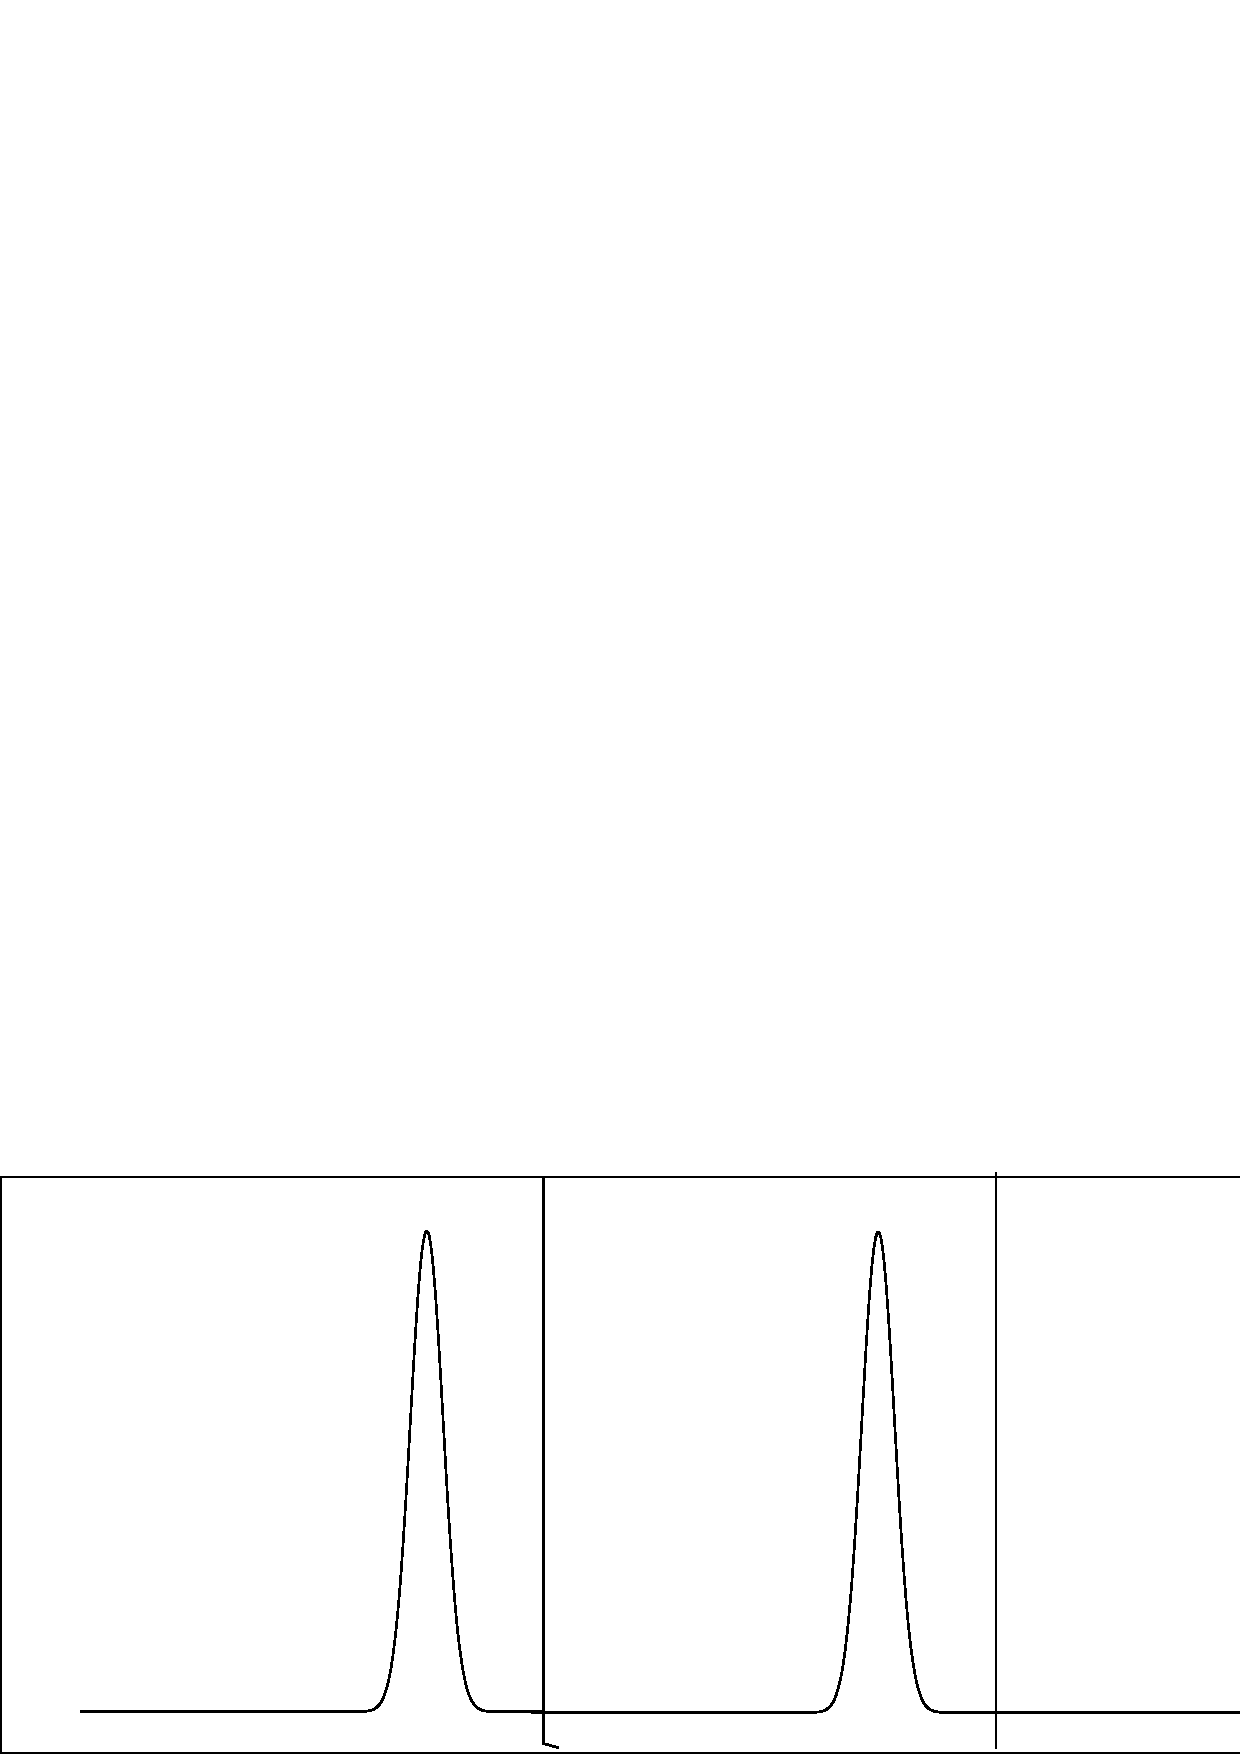
\includegraphics[width=7cm]{pulses.pdf}
  \caption{Pulses}
  \label{fig:pulses}
\end{figure}
\begin{figure}[H]
  \centering
  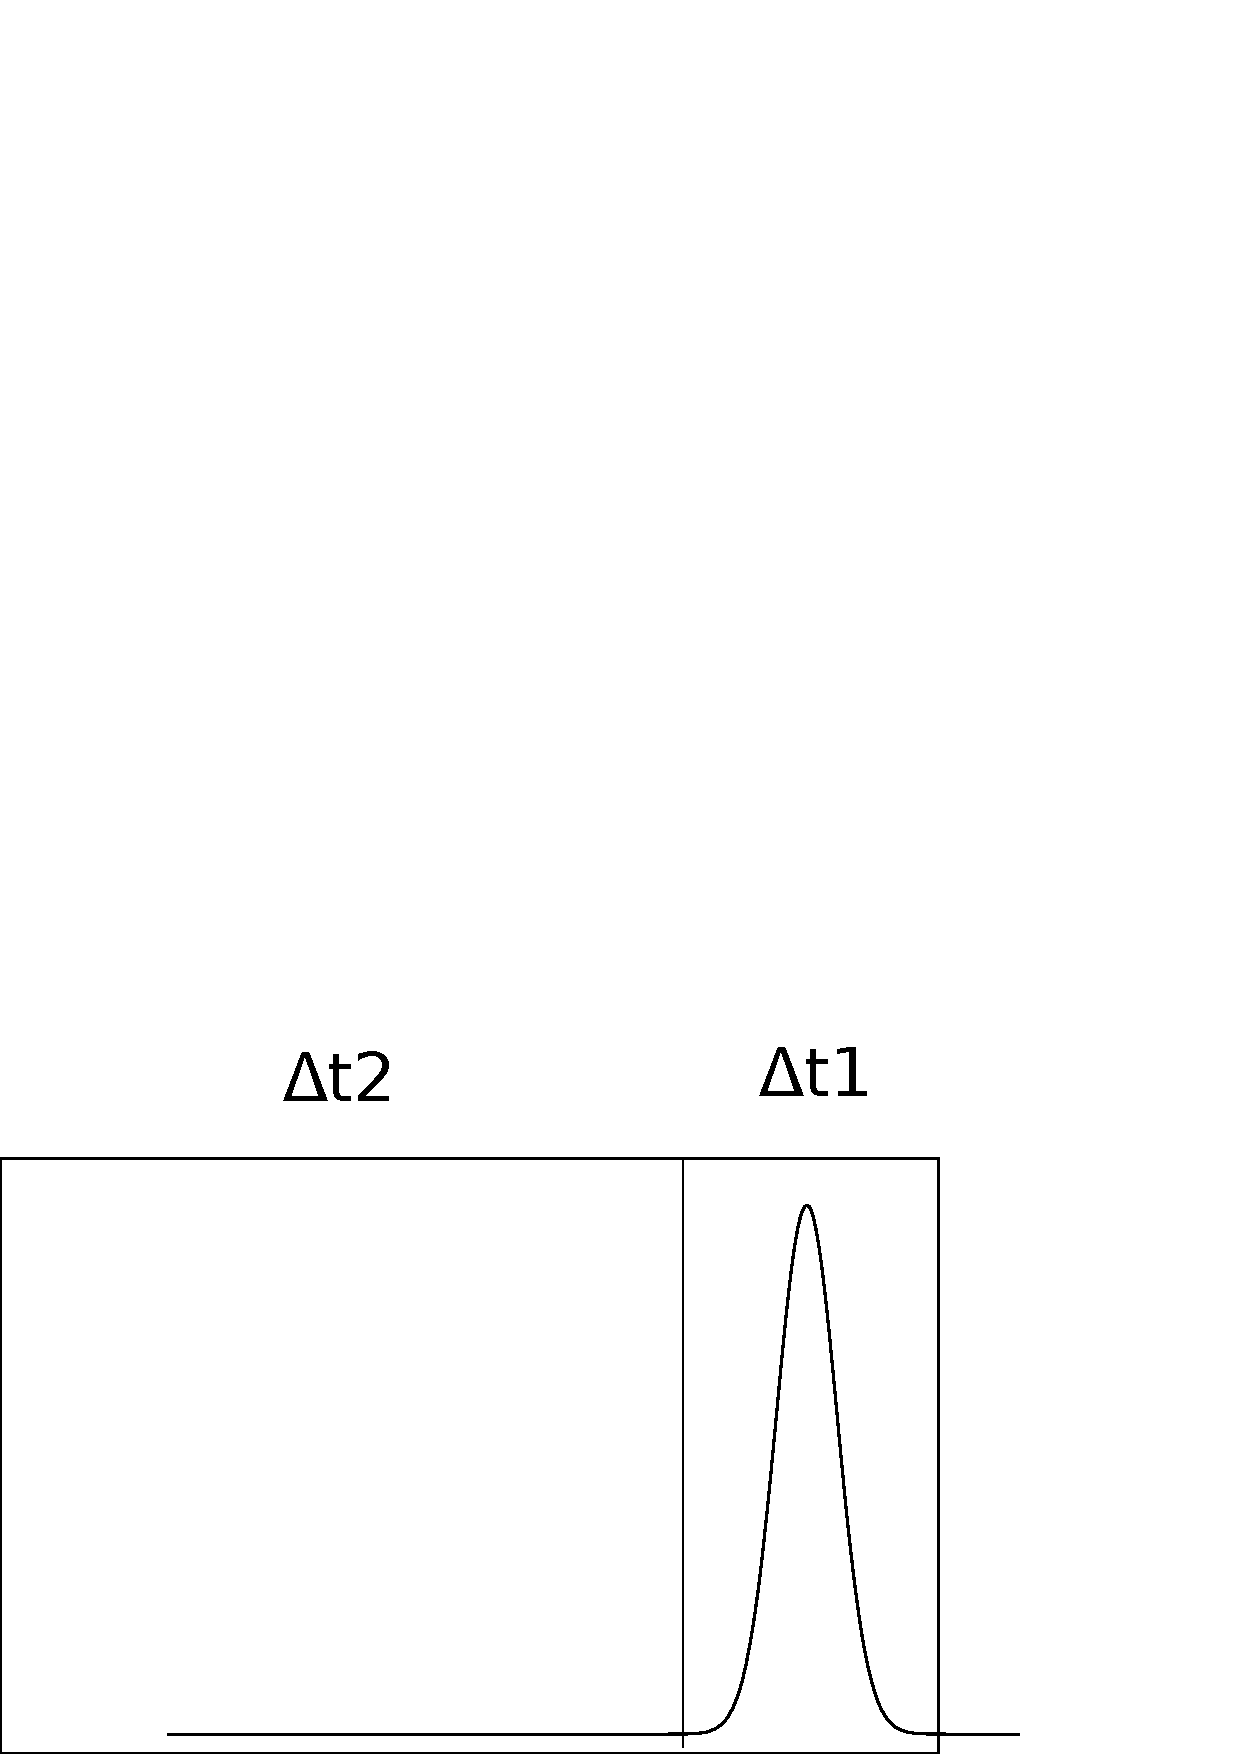
\includegraphics[width=6cm]{pulse.pdf}
  \caption{Pulse}
  \label{fig:pulse}
\end{figure}
The laser pulse train can be divided in to segments as fig.\ref{fig:pulses} shows. The time segment between two adjacent pulses can be further divided into two parts, one with duration $\Delta t_1$ which contain the laser field , another with duration $\Delta t_{2}$ has negligible electric field, as fig.\ref{fig:pulse} shows.\\

Suppose the unraveled density matrix is $\tilde{\rho}(0)$ just before the pulse. Define two super operator as follow:
\[
\tilde{\rho}(\Delta t_1) = \mathcal{P}^{\prime} \left[ \tilde{\rho}(0) \right]
\]
\[
\tilde{\rho}(\Delta t_1+\Delta t_2) = \mathcal{P} \left[\tilde{\rho}(\Delta t_{1})\right] = \mathcal{P} \mathcal{P}^{\prime} \left[\tilde{\rho}(0)\right]
\]

Since there is no electric field in the period $\Delta t_1<t<\Delta t_1+\Delta t_2$, the motion equation is $\dot{\tilde{\rho}} = \mathcal{A} \left[\tilde{\rho}\right]$. So $\tilde{\rho}(\Delta t_1+\Delta t_2) = e^{i \mathcal{A} \Delta t_{2}} \left[ \tilde{\rho}(\Delta t_{1}) \right] $, the exponential of super operator in this case can be calculated just as the matrix exponential.
\[
\mathcal{P} = e^{i \mathcal{A} \Delta t_2}
\]

The part with electric field, $\mathcal{P}^{\prime}$ can be solve with perturbation method. Define $\tilde{\rho}_n (t)$ as the $n$th order solution of equation of motion $\dot{\tilde{\rho}} = \left( A + B E_{env}(t) \right) \left[ \tilde{\rho} \right] $ where $0< t < \Delta t_{1}$. Define another super operator $F(t)_{n} \tilde{\rho}(0) = \tilde{\rho}_{n}(t)$, that transfer the initial condition $\tilde{\rho}(0)$ into $n$th order solution of time $t$, $\tilde{\rho}_n (t)$. (ELABORATE BETTER)% and $G_{n}(t) \zeta(0) = \dot{\zeta_{n}(t)}$. $\frac{d F_{n}(t)}{dt} = G_{n}(t)$.\\

If the initial condition of density matrix $\tilde{\rho}(0)$ is known. $\tilde{\rho}_{0} (t) = e^{i A t} \tilde{\rho}(0)$. The next order of $\tilde{\rho}$ can be obtain by:
\begin{equation}
  \label{eq:perturb}
  \tilde{\rho}_{n+1}(t) = \int_0^{t} \left( \mathcal{A}+\mathcal{B} E_{env}(\tau) \right) \tilde{\rho}_n(\tau)\:d\tua, 0<t<\Delta t_1
\end{equation}
substitute $\tilde{\rho}_n(t)$ for $F_n(t)\tilde{\rho}(0)$,eq.\ref{eq:perturb} becomes:
\begin{equation}
  F_{n+1}(t)\tilde{\rho}(0) = \int_0^{t} \left( \mathcal{A}+\mathcal{B} E_{env}(\tau) \right) F_n(\tau)\tilde{\rho}(0)\:d\tau, 0<t<\Delta t_1
\end{equation}
remove the constant array $\tilde{\rho}(0)$ which is the initial condition from both side:
\begin{equation}
  \label{eq:f}
  F_{n+1}(\Delta t_1) = \int_0^{\Delta t_1} \left( \mathcal{A}+\mathcal{B} E_{env}(t) \right) F_n(t)\:dt
\end{equation}
$F_0(t) = e^{-iAt}$ and $F_{n}(0)$ is identity matrix $I$, eq.\ref{eq:f} is independent of initial condition $\tilde{\rho}(0)$. So $\mathcal{P}^\prime = \lim_{n\rightarrow \infty}F_{n}(\Delta t_{1})$.\\

The evolution of density matrix can be calculated with $\mathcal{P}\mathcal{P}^\prime \left[ \tilde{\rho} \right]$. After $n$ pulses the density matrix become $\left(\mathcal{P} \mathcal{P}^{\prime} \right)^{n} \left[ \tilde{\rho} \right]$. The steady state of the system can be calculate with $\left(\mathcal{P} \mathcal{P}^{\prime} \right)\left[ \tilde{\rho}_{\mbox{steady state}} \right] = \tilde{\rho}_{\mbox{steady state}}$.
% find how to write super operator $h \[ \rho\]$



\section{Numerical Results}
A program based on previous algorithm is written with Enthought Python Distribution (EPD) \todo{finde citation}\cite{scipy} embedded with some performance critical part written in C linked against Intel Math Kernel Library (MKL). The program is executed on a computer cluster with 24GB of memory on every node.\\

In the calculation, data and parameters from Ref.\cite{Steck2003} is used. \todo{Need to find original data, since D Line data is not a review paper}\\

All Zeeman sublevels in P and S orbital are taking into account. Which is 32 levels in $D_1$ case and 48 levels in $D_2$ case. With 48 levels, density matrix has 2304 elements and super operator has 5308416 elements. The perturbation algorithm require a super operator for every time step, so the algorithm require lots of memory.\\

In $D_1$ case the carrier frequency is tuned to frequency difference between $6^2S_1/2, F=3$ and $6^2P_{1/2}, F=3$, in $D_2$ case the carrier frequency is tuned to $6^2S_1/2$ $F=3$ and $6^2P_{3/2}$ $F=3$. Repetition rate is set to $0.919263177 \giga\hertz$ which is $\frac{1}{10}$ of the frequency between $6^2S_1/2$ $F=3$ and $6^2S_1/2$ $F=4$. The laser is circular polarized ($\sigma = +1$). No magnetic field is applied.\\

The decay rate $\Gamma$ is set to $7 \times 10^8 \hertz$ to fit the experiment condition. The FWHM of laser pulse is $-27.7\femto\second$, with a Gaussian envelope $C e^{ - \frac{t^2}{2 \sigma^{2}} }$, where $\sigma = 20 \times 10^{-15} \second$.\\
% $\gamma	= 5\hertz$ and $\gamma = 1000\hertz$ is calculated.\\
%why select these parameters

\subsection{Three, four and five level model}
The algorithm presented in previous section is used to calculate the comb CPT signal of these models. The difference between three level model and other model is that since there is no trap state in the tree level model, CPT signal can occurred without considering ground state relaxation rate. However, in four or five level model, with ground state relaxation rate set to zero, all the atoms is trapped in the trap state, leaves no atom in the higher energy state, regardless of repetition rate. as shown in figure \ref{fig:four_level_result_nogamma}. In the five level model that model the $D_2$ system, all atoms is trapped in the trap state and the $F=5, m_f=5$ state, so the higher state population become a constant which is independent of repetition rate, as shown in figure \ref{fig:five_level_result_nogamma}.\\
 %explain how laser frequency is shifted
\begin{figure}[H]
  \centering
  \subfigure[Four level system result without $\gamma$]{
  \includegraphics[width=0.4\textwidth]{small_system/four_level_1000_no_gamma.png}
  \label{fig:four_level_result_nogamma}
}\\
  \subfigure[Five level system result without $\gamma$]{
  \includegraphics[width=0.4\textwidth]{small_system/five_level_10_nogamma.png}
  \label{fig:five_level_result_nogamma}
}
  \caption{Comb CPT signal: temporal evolution of P orbital population with 0 ground state relaxation rate, the figures plot the higher energy level population against time and frequency shift of the laser. Only the higher energy states are plotted because the fluorescence observed in experiment is proportional to the higher state population.}
  \label{fig:nogamma}
\end{figure}

\begin{figure}[H]
  \centering
  \subfigure[Three level system]{
    \includegraphics[width=0.3\textwidth]{small_system/three_level_1000.png}
  \label{fig:three_level_result}
}
  \subfigure[Four level system]{
    \includegraphics[width=0.3\textwidth]{small_system/four_level_1000.png}
  \label{fig:four_level_result}
}
  \subfigure[Five level system]{
    \includegraphics[width=0.3\textwidth]{small_system/five_level_1000.png}
  \label{fig:five_level_result}
}
  \caption{numerical result: P orbital population plot against time and repetition rate. The graph shown the temporal evolution of comb CPT signal}
  \label{fig:small_system_result}
\end{figure}

\subsection{Effect of ground state relaxation rate $\gamma$}
The linewidth and contrast of $D_2$ line comb CPT signal is plotted in figure \ref{fig:gamma_relation}. As figure \ref{fig:gamma_relation} shows, line width is proportional to the ground state relaxation rate $\gamma$. And as $\gamma$ increase, contrast decrease monotonously. %physical explanation
\begin{figure}[H]
  \centering
  \subfigure[linewidth vs $\gamma$]{
    \includegraphics[width=0.4\textwidth]{d2_gamma/linewidth.eps}
    \label{fig:linewidth_gamma}
  }\\
  \subfigure[contrast vs $\gamma$]{
    \includegraphics[width=0.4\textwidth]{d2_gamma/contrast.eps}
    \label{fig:contrast_gamma}
  }
  \caption{d2 line linewidth and contrast vs $\gamma$}
  \label{fig:gamma_relation}
\end{figure}

\subsection{Comparison Of Cw Laser And Pulse Laser}
We calculated the line width, contrast and light shift of both comb CPT and CW CPT signal of $D_1$ and $D_2$ absorption spectrum. And we plot these results against the average power of laser. The value of ground state relaxation rate $\gamma$ is set to $5 \hertz$ to fit the experimental data. In this comparison, the repetition rate of pulse laser is modulated. And the frequency of both lasers in CW CPT $\Lambda$ is modulated, to simulate the condition of experiment which use AMO modulation \todo{check}. The frequency of two lasers change in different direction at the same time. For example if the frequencies of two lasers are $\nu_1$ and $\nu_2$, the frequencies after the modulation become $\nu_1+\delta$ and $\nu_2-\delta$.
  \begin{figure*}
  \subfigure[$D_1$ cw and pulse linewidth]{
    \includegraphics[width=0.4\textwidth]{d1_cw_p/linewidth.eps}
    \label{fig:d1linewidth}
  }
  \subfigure[$D_1$ cw and pulse contrast]{
    \includegraphics[width=0.4\textwidth]{d1_cw_p/contrast.eps}
    \label{fig:d1contrast}
  }\\
  \subfigure[$D_1$ cw and pulse light shift]{
    \includegraphics[width=0.4\textwidth]{d1_cw_p/lightshift.eps}
    \label{fig:d1lightshift}
  }
  \subfigure[$D_2$ cw and pulse linewidth]{
    \includegraphics[width=0.4\textwidth]{d2_cw_p/linewidth.eps}
    \label{fig:d2linewidth}
  }\\
  \subfigure[$D_2$ cw and pulse contrast]{
    \includegraphics[width=0.4\textwidth]{d2_cw_p/contrast.eps}
    \label{fig:d2contrast}
  }
  \subfigure[$D_2$ cw and pulse light shift]{
    \includegraphics[width=0.4\textwidth]{d2_cw_p/lightshift.eps}
    \label{fig:d2lightshift}
  }
  \caption{Difference between CW and comb CPT signal}
  \label{fig:cwp}
\end{figure*}
The simulation results of CW and pulse laser CPT signal are compared. The results are in figure \ref{fig:cwp}. For both $D_1$ and $D_2$ CPT line width are smaller for comb CPT signal, as shown in figure \ref{fig:d1linewidth} and \ref{fig:d2linewidth}. Line width of comb CPT signal is under $3 \hertz$ in simulated laser power range, while CW CPT line width is much larger. As for contrast, for $D_1$ CPT, contrast increase as laser power increase for both CW and comb CPT signal, see figure \ref{fig:d1contrast}. However for $D_2$ case, contrast of CW CPT signal drop after certain laser power, as shown in figure \ref{fig:d2contrast}}, that is because higher laser power causes the population of trap state ($F=5, m=5$ for $\sigma = 1$) to rise ($10^{-6}$), which create decoherence while it relax. This phenomenon is also found by Vanier et al. \cite{Vanier1998}. The population of trap state in pulse laser case is much smaller (of order $1 \times 10^{-10}$). Pulse CPT signal also has a much smaller light shift compare to CW CPT, as shown in figure \ref{fig:d1lightshift} and figure \ref{fig:d2lightshift}.\todo{explain jitter}

\section{Conclusions}
In conclusion we present an effective algorithm to calculate comb CPT signal taking account of all Zeeman sublevels. The line width and light shift of comb CPT signal is much smaller its counterpart CW CPT signal. Some features present in full Zeeman sublevels simulation do not appear in four or five level model\doto{verify}.
\bibliography{reference}{}
\bibliographystyle{plain}
\end{document}








